\begin{enumerate}
\item Se experimenta con lograr la FFT con solo una reducción de orden. Para lo anterior se escribe la función $X = DFTdc(x)$, la cual implementa una etapa del algoritmo recursivo de la FFT y luego utiliza la función $DFTsum$ para obtener la DFT de las señales de muestras pares e impares.

El código escrito para la función $DFTdc$ se muestra a continuación:
\begin{lstlisting}[language = octave]
function X = DFTdc(x)
    N  = length(x);
    W  = exp(-1j*2*pi/N);
    Wk = W.^(0:(N/2-1));
    
    x0 = zeros(1,N/2);
    x1 = zeros(1,N/2);
    
    for i = 1:N/2
        x0(i) = x(2*i-1); %OBS "par"   1,3,5,... en MATLAB
        x1(i) = x(2*i);   %OBS "impar" 2,4,6,... en MATLAB       
    end
    
    X0 = DFTsum(x0); X1 = DFTsum(x1);
    
    X_izq = X0 + Wk.*X1;
    X_der = X0 - Wk.*X1;
    
    X = [X_izq X_der];    
end
\end{lstlisting}

Posteriormente se utiliza la función generada para obtener la DFT de 3 señales de prueba:
\begin{itemize}
    \item Señal a: $x(n) = \delta(n)$
    \item Señal b: $x(n) = 1$
    \item Señal c: $x(n) = e^{-j\frac{2\pi n}{8}}$
\end{itemize}

Las magnitudes de la DFT obtenidas con la función para las señales de prueba se muestran en la figura \ref{p6_1dft}, donde además se muestran las magnitudes de la DFT utilizando el comando $fft$ de MATLAB con fines comparativos. Como era de esperarse, no se aprecian diferencias visuales en los resultados obtenidos.

\begin{figure}[H]
    \centering
    \includegraphics[width = .98 \linewidth]{Figuras/p6_1dft.eps}
    \caption{Comparación entre magnitudes de DFT obtenidas con función $DFTdc$ y $fft$ en MATLAB.}
    \label{p6_1dft}
\end{figure}

Finalmente se obtiene el tiempo de procesamiento para la función $DFTdc$ y $fft$, obteniendo:
\begin{itemize}
    \item $DFTdc$: $3.64123\cdot 10^{-5}~s$ 
    \item $fft$:   $9.84100\cdot 10^{-7}~s$
\end{itemize}
Se aprecia que la implementación de la $fft$ de MATLAB es muy superior a la función generada al calcular una DFT de 8 puntos.

\item Se experimenta con FFTs de 2, 4 y 8 puntos, programando las funciones $FFT2, FFT4$ y $FFT8$, las cuales corresponden a implementaciones explícitas de las ecuaciones del algoritmo fft.

En primer lugar se implementa la función $FFT2$, a partir de las ecuaciones:
\begin{align*}
    X^{(2)}(0) &= x(0) + x(1)\\
    X^{(2)}(1) &= x(0) - x(1)
\end{align*}
Donde $X^{(2)}$ corresponde a la DFT de la señal $x$, la cual tiene 2 puntos.

El código escrito para la función $FFT2$ se muestra a continuación:
\begin{lstlisting}[language = octave]
function X = FFT2(x)
    X = zeros(1,2);
    
    X(1) = x(1) + x(2);
    X(2) = x(1) - x(2);
end
\end{lstlisting}

Las funciones $FFT4$ y $FFT8$, corresponden a la implementación con $N=4$ y $8$ respectivamente de las siguientes ecuaciones:
\begin{align*}
    X^{(N)}(k)   &= X_0^{(N/2)}(k) + W^k_N X_1^{(N/2)}(k)\\
    X^{(N)}(N/2+k) &= X_0^{(N/2)}(N/2+k) - W^k_N X_1^{(N/2)}(N/2+k)
\end{align*}
Donde
\begin{itemize}
    \item $X^{(N)}$ corresponde a la DFT de la señal $x$, la cual tiene $N$ puntos 
    \item $X_0^{(N/2)}(k)$ y $X_0^{(N/2)}(k)$ corresponden a la DFT de la señal de muestras pares e impares de $x$.
    \item $W_N = e^{(-j2\pi/N)}$ corresponde al factor de twiddle.
\end{itemize}

La implementación de $FFT4$, se muestra a continuación:
\begin{lstlisting}[language = octave]
function X = FFT4(x)
    X = zeros(1,4);
    
    x0 = [x(1) x(3)]; %Muestras "pares"
    x1 = [x(2) x(4)]; %Muestras "impares"
    
    X0 = FFT2(x0);
    X1 = FFT2(x1);
    
    X(1) = X0(1) +   (1)*X1(1);
    X(2) = X0(2) + (-1j)*X1(2);    
    
    X(3) = X0(1) -   (1)*X1(1);
    X(4) = X0(2) - (-1j)*X1(2);    
end
\end{lstlisting}

La implementación de $FFT8$ se muestra a continuación:
\begin{lstlisting}[language = octave]
function X = FFT8(x)
    X = zeros(1,8);
    
    x0 = [x(1) x(3) x(5) x(7)]; %Muestras "pares"
    x1 = [x(2) x(4) x(6) x(8)]; %Muestras "impares"
    
    X0 = FFT4(x0);
    X1 = FFT4(x1);
    
    X(1) = X0(1) +               (1)*X1(1);
    X(2) = X0(2) +   (exp(-1j*pi/4))*X1(2);
    X(3) = X0(3) +             (-1j)*X1(3);
    X(4) = X0(4) + (exp(-1j*3*pi/4))*X1(4);
    
    X(5) = X0(1) -               (1)*X1(1);
    X(6) = X0(2) -   (exp(-1j*pi/4))*X1(2);
    X(7) = X0(3) -             (-1j)*X1(3);
    X(8) = X0(4) - (exp(-1j*3*pi/4))*X1(4);
end
\end{lstlisting}

Posteriormente se utiliza la función $FFT8$ generada para obtener la DFT de 3 señales de prueba del punto anterior.

Las magnitudes de la DFT obtenidas con la función para las señales de prueba se muestran en la figura \ref{p6_2dft}, donde además se muestran las magnitudes de la DFT utilizando el comando $fft$ de MATLAB con fines comparativos. Como era de esperarse, no se aprecian diferencias visuales en los resultados obtenidos.

\begin{figure}[H]
    \centering
    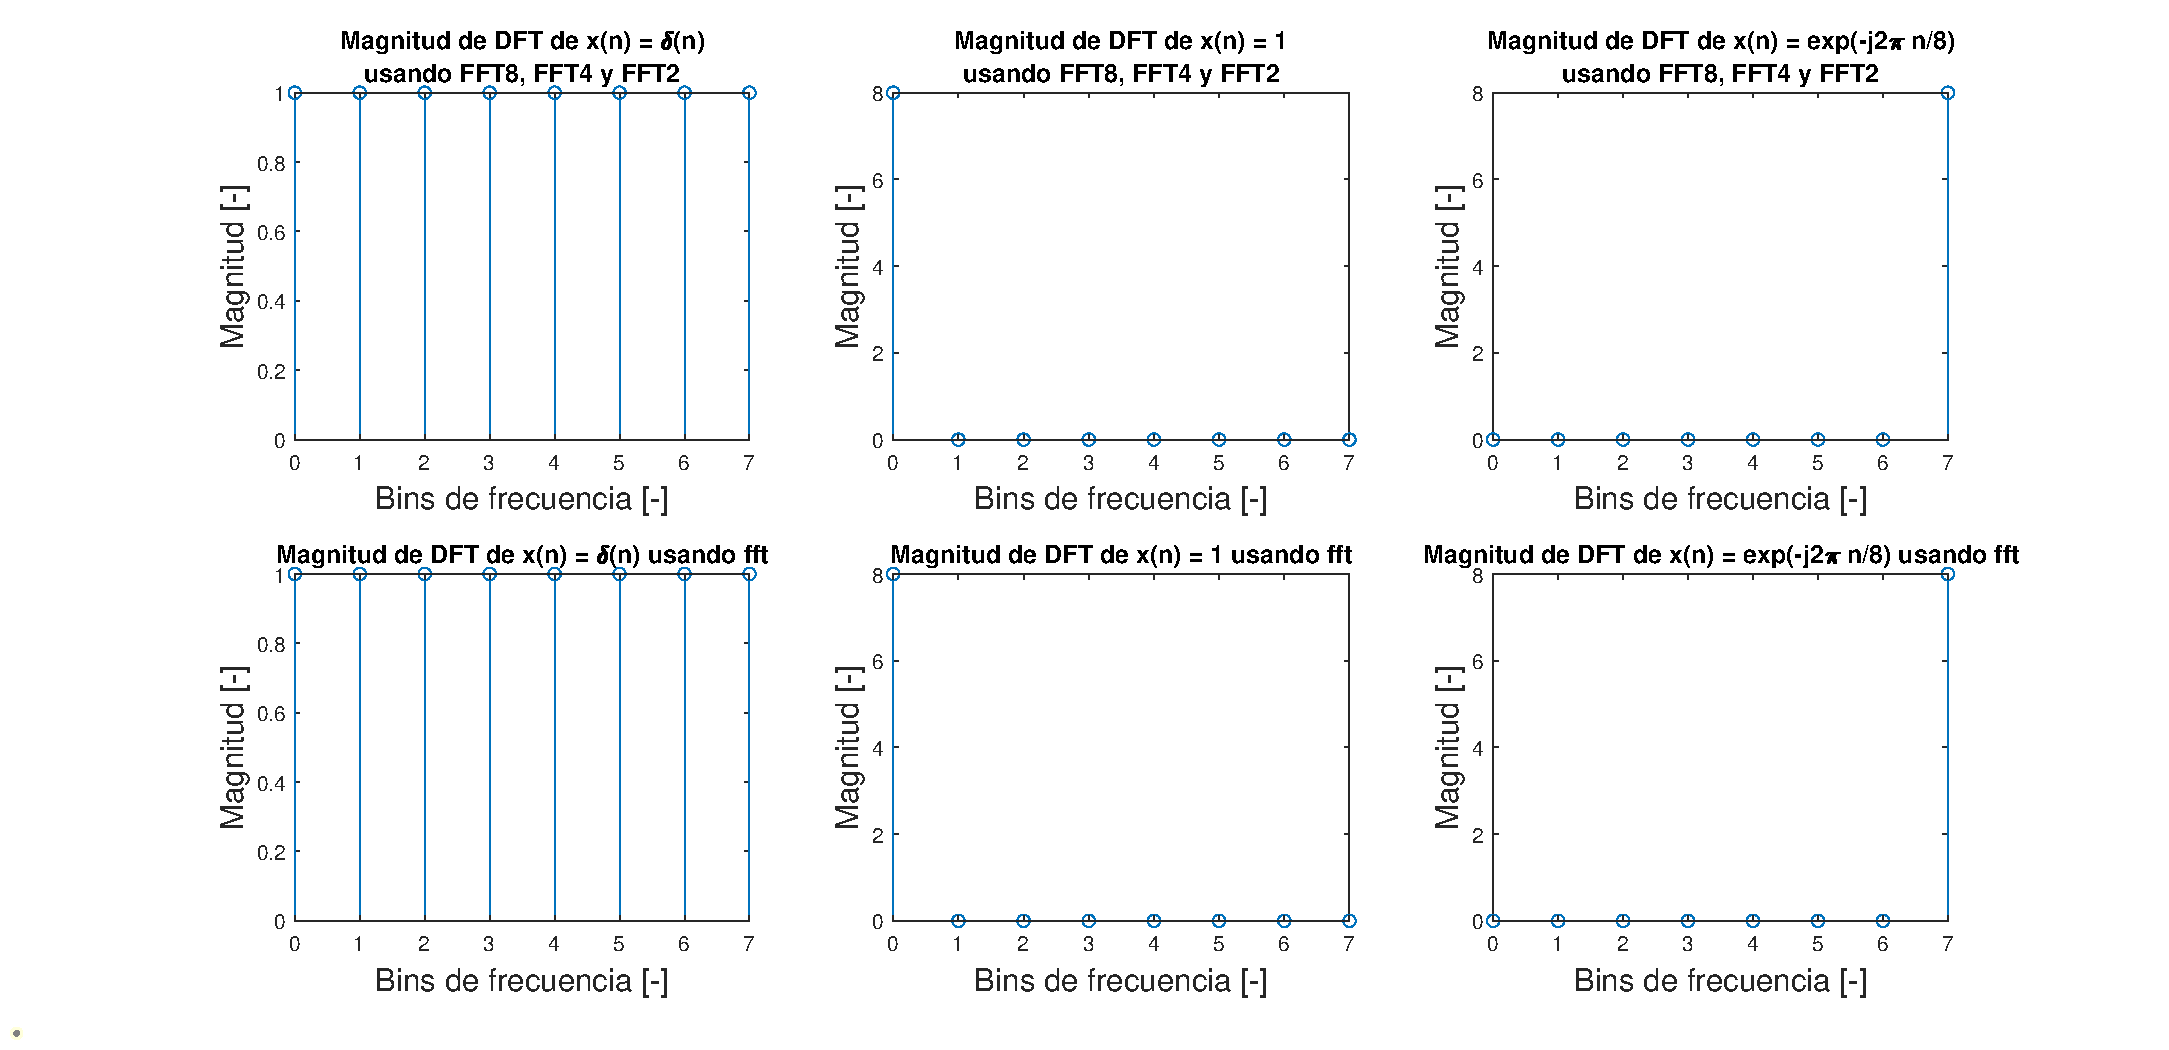
\includegraphics[width = .98 \linewidth]{Figuras/p6_2dft.eps}
    \caption{Comparación entre magnitudes de DFT obtenidas con función $FFT8$ y $fft$ en MATLAB.}
    \label{p6_2dft}
\end{figure}

Finalmente se obtiene el tiempo de procesamiento para la función $FFT8$ y $fft$, obteniendo:
\begin{itemize}
    \item $FFT8$: $1.63822\cdot 10^{-5}~s$ %3.64123e-05 seg 
    \item $fft$:  $7.75409\cdot 10^{-7}~s$ %9.84100e-07 seg
\end{itemize}
Se aprecia que la implementación de la $fft$ de MATLAB sigue siendo muy superior a la función generada al calcular una DFT de 8 puntos. Sin embargo, cabe destacar que hubo una mejora con respecto al algoritmo $DFTdc$.

\item Se crea la función recursiva $X = fft\_stage(x)$, la cual aplica el algoritmo FFT para señales de largo $2^{n}$. El código se muestra a continuación:

\begin{lstlisting}
function X = fft_stage(x)
    N = length(x);
    
    if (N == 2)
        X = FFT2(x);
        return
    else    
        x0    = zeros(1,N/2); x1    = zeros(1,N/2);        
    
        for i = 1:N/2
            x0(i) = x(2*i-1); %OBS "par"   1,3,... en MATLAB
            x1(i) = x(2*i);   %OBS "impar" 2,4,... en MATLAB       
        end
    
        W = exp(-1j*2*pi/N);  Wk = W.^(0:(N/2-1));        
        X0 = fft_stage(x0) ;  X1 = fft_stage(x1) ; 
    
        X_izq = X0 + Wk.*X1;
        X_der = X0 - Wk.*X1;
    
        X = [X_izq X_der];
    end
end
\end{lstlisting}

Se utiliza el comando \texttt{timeit} de MATLAB para comparar el tiempo de procesamiento al utilizar de entrada la señal del punto \textbf{4.3}, considerando largos de $N = [2^{10}, 2^{11}, \dots , 2^{19}]$. Los gráficos con los tiempos de cómputo se muestran en la figura \ref{p6_3cmp}
\begin{figure}[H]
    \centering
    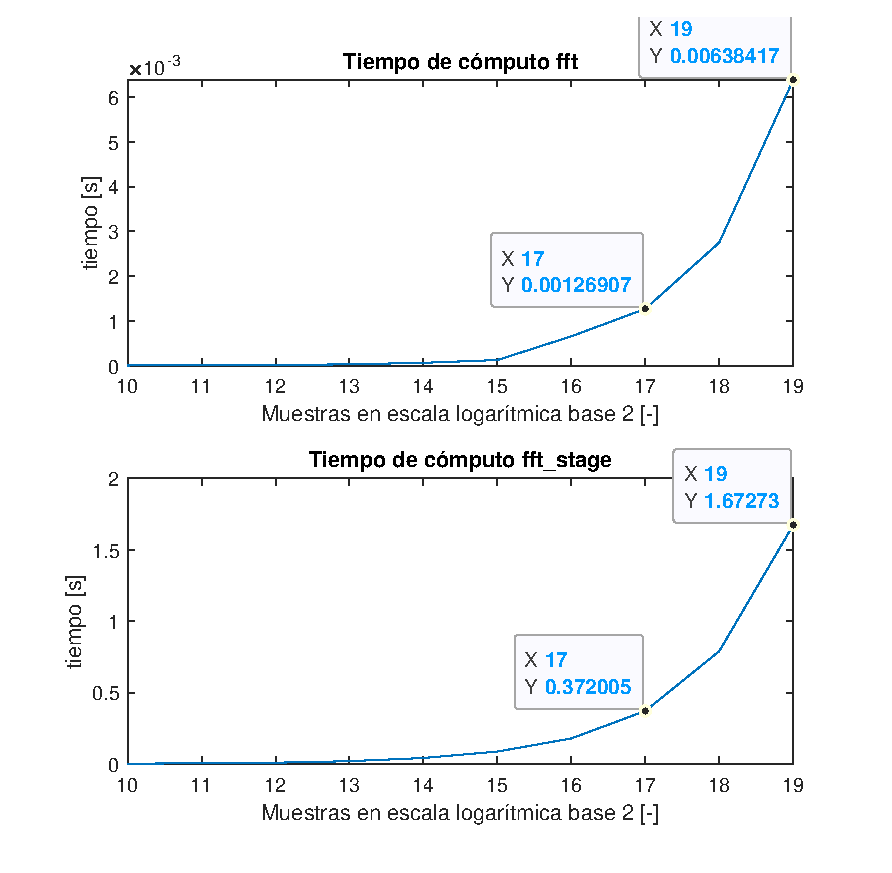
\includegraphics[width = .98 \linewidth]{Figuras/p6_3_cmp.eps}
    \caption{Tiempos de cómputo de función $fft\_stage$ y $fft$ para distintos largos de señal.}
    \label{p6_3cmp}
\end{figure}

De los resultados de tiempo de cómputo obtenidos se concluye que:
\begin{itemize}
    \item La implementación de MATLAB es muy superior a $fft\_stage$. La razón entre el tiempo de cómputo de la $fft$ con respecto a $fft\_stage$ es del orden de $10^-3$. 
    \item La curva de tiempo de cómputo en ambos algoritmos son similares.
\end{itemize}
\end{enumerate}